\documentclass[twocolumn]{article}
\usepackage{graphicx} % Required for inserting images
\usepackage{amsmath}
\usepackage{subcaption}
\usepackage[hyphens]{url}
\usepackage{hyperref}
\hypersetup{breaklinks=true}

\urlstyle{same}

\pagenumbering{gobble}

\title{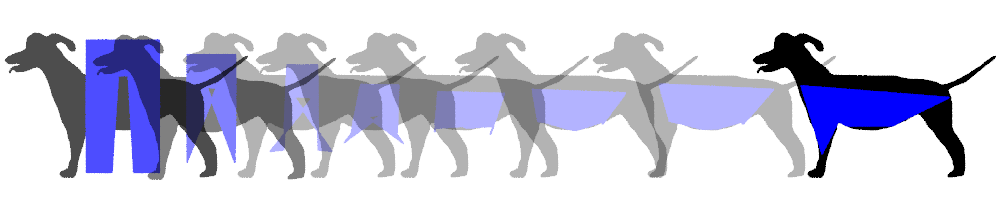
\includegraphics[width=0.7\textwidth]{img/teaser.png}\\A Jalgorithm for Japplying Jeans to Jobjects}
\author{Dave Pagurek}
\date{March 2023}

\begin{document}

\maketitle

\begin{abstract}
    For years, society has been plagued by the lack of a conclusive answer to the question of how arbitrary things would wear jeans, if they wore jeans. This paper proposes a jalgorithm to determine the mathematically optimal configuration of pants on a silhouette, leveraging recent insights in the fields of computer vision and differentiable rendering.
\end{abstract}

\section{Introduction}

In recent years, the internet has been ruminating over the question of how various objects would wear pants, if they hypothetically wore pants.~\cite{know_your_meme} It began in 2015 using a dog as the object in question,~\cite{utopian_raspberry} with other objects such as  humans on their hands and knees~\cite{reddit} or pants themselves~\cite{twitter} being discussed later. 

Despite being in the public discourse for nearly a decade, no conclusions have been reached. The authors believe this is due to a lack of a principled approach to the study of pants-wearing. This paper aims to rectify the situation by proposing a formula to score the quality of the application of pants to an object, and writing software to optimally apply pants under this system.

\section{Background}

Gradient-based optimization has been a subject of study in mathematics for a long time. The core idea is that if one has an objective function one wishes to maximize or minimize, one can use the gradient of the output with respect to the function's inputs to determine how to adjust the inputs in order to move the output closer to the desired outcome. There are many algorithms, including Adam optimization~\cite{Adam}, to update inputs in this manner using gradient information.

Differentiable rendering is a technique in the world of computer graphics and computer vision that enables gradient-based optimization of functions involving rendering of images. If the rendering process is itself differentiable, then one could, for example, optimize the representation of a 3D scene such that it matches a reference photo when rendered.~\cite{liu2019softras,liu2020general} The diffvg library~\cite{Li:2020:DVG} provides a differentiable vector graphics renderer, allowing one to optimize 2D vector shapes such as lines, curves, and polygons to produce desired visuals.

\section{Method}
\label{sec:method}

\subsection{Algorithm}

Our pants-fitting jalgorithm takes as input a vector shape representing a silhouette on which one wants to apply pants. We rasterize this to a 256$\times$256-pixel image, concerning ourselves only with the alpha channel. We will refer to this one-channel silhouette image as the 256$\times$256 matrix $S$.

We then create a polygon representing the pants we want to fit onto the silhouette, whose vertex positions $X$ we will optimize. We initialize its vertices to $\mathbf{X}$, the shape of prototypical jeans, shown in Figure~\ref{fig:prototypical}. We then solve for the vertices $\hat{X}$ that minimize pants-fitting loss, $l(X)$, described in detail in Section~\ref{sec:loss}, using Adam optimization~\cite{Adam} and gradients provided via diffvg~\cite{Li:2020:DVG} vector rendering and Torch~\cite{paszke2017automatic} for 100 iterations:
\begin{equation}
    \hat{X} = \text{argmin}_X l(X)
\end{equation}

\begin{figure}
    \centering
    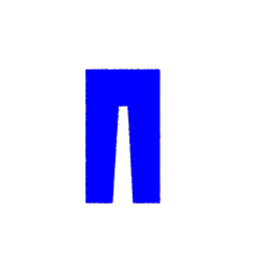
\includegraphics[width=0.38\textwidth]{img/init.png}
    \caption{Prototypical jeans: $\mathbf{X}$, the initial pants shape we apply to objects.}
    \label{fig:prototypical}
\end{figure}

\subsection{Loss Function}
\label{sec:loss}

Our loss function is motivated by insights from the authors' multuple decades of pants-wearing experience. We propose the following rules, which we then will encode mathematically:
\begin{enumerate}
    \item \textbf{Duality of man:} Pants should bisect the silhouette of the wearer through its center, covering half its area.
    \item \textbf{No-stretch jeans:} Pants, when applied to the wearer in rest position, should not be so deformed that they no longer resemble prototypical jeans.
    \item \textbf{(Topologically) torn jean avoidance:} Limbs should only go through the open ends of pants, and similarly, closed ends of pants should not intersect limbs.
    \item \textbf{Dress code compliance:} Pants should be on the body of the wearer, not off of it.
\end{enumerate}

From Rule~1, we get the following loss terms, where $x_\text{topleft}$ and $x_\text{topright}$ correspond to the endpoints of the waistband of prototypical jeans, and $J(X)$ is the 256$\times$256 matrix of the rendered alpha channel of the jeans vertices $\mathbf{X}$. $L_\text{center}$ incentivizes waistbands that go through the center of the silhouette, and $L_\text{coverage}$ incentivizes jeans that cover half of the silhouette.
\begin{align}
    L_\text{center} &= \left\Vert \frac{x_\text{topleft} + x_\text{topright}}{2} - \begin{bmatrix}0.5 \\ 0.5\end{bmatrix} \right\Vert^2 \\
    L_\text{coverage} &= \left(\frac{1}{2} - \frac{\sum_{i,j} \max{\left(\left(S - J(X)\right)_{ij}, 0\right)}}{\sum_{i,j} S_{ij}} \right)^2
\end{align}

From Rule~2, we get the loss term $L_\text{rigid}$, which incentivizes the jean points $X$ to be as close as possible to an affine transformation of the prototypical jean points $\mathbf{X}$ by finding the error of the least-squares-minimal transformation $T$ that describes the relation between $X$ and $\mathbf{X}$.
\begin{align}
    L_\text{rigid} &= \left\Vert X - T\mathbf{X}\right\Vert^2,\\
    T &= \begin{bmatrix}
        \hat{p}_1 & \hat{p}_2 & \hat{p}_3 \\
        \hat{p}_4 & \hat{p}_5 & \hat{p}_6 \\
        0 & 0 & 1
    \end{bmatrix},\\
    \hat{p} &= \operatorname{argmin}_p \left\Vert
    \begin{bmatrix}\mathbf{X}_{0,1} \\ \mathbf{X}_{1,1} \\ \vdots \\ \mathbf{X}_{0,n} \\ \mathbf{X}_{1,n}\end{bmatrix} -
    \begin{bmatrix}
        \multicolumn{2}{c}{X_{0:1,1}} & 1 & 0 & 0 & 0 \\
        0 & 0 & 0 & \multicolumn{2}{c}{X_{0:1,1}} & 1 \\
         \multicolumn{6}{c}{\vdots} \\
        \multicolumn{2}{c}{X_{0:1,n}} & 1 & 0 & 0 & 0 \\
        0 & 0 & 0 & \multicolumn{2}{c}{X_{0:1,n}} & 1
    \end{bmatrix}
    p
    \right\Vert^2
\end{align}

From Rule~3, we get the terms $L_\text{open}$ and $L_\text{closed}$, terms incentivizing open and closed edges of the jeans respectively to and to not intersect the silhouette, and $L_\text{inter}$, incentivizing edges to not intersect each other. We refer to the set of all edges as $E(X)$, and the of open and closed edges as $E_o(X)$ and $E_c(X)$. The rendered alpha channel of an edge with stroke thickness of 5 is referred to as $R(e)$.
\begin{align}
    L_\text{open} &= \frac{-\sum_{i,j} R(E_o(X))_{ij} S_{ij}}{\sum_{i,j} R(E_o(X))_{ij}} \\
    L_\text{closed} &= \frac{\sum_{i,j} R(E_c(X))_{ij} S_{ij}}{\sum_{i,j} R(E_c(X))_{ij}} \\
    L_\text{inter} &= \sum_{\{e_1, e_2\} : \binom{E(X)}{2}} \frac{\sum_{i,j} R(e_1)_{ij} R(e_2)_{ij}}{ \sum_{i,j} \min{\left( R(e_1)_{ij} + R(e_2)_{ij}, 1 \right)}}
\end{align}

From Rule~4, we get $L_\text{inside}$, discouraging the pants from being off the silhouette:
\begin{equation}
    L_\text{inside} = \frac{\sum_{i,j} \max{\left( J(X)_{ij} - S_{ij}, 0 \right)}}{\sum_{i,j}J(X)_{ij}}
\end{equation}

We take a weighted sum over all the loss terms to get the final loss function:
\begin{equation}
    l(X) = \sum_{i} k_i L_i
\end{equation}

For our results, we used the following weights:
\begin{align*}
    k_\text{center} &= 50, \\
    k_\text{coverage} &= 100, \\
    k_\text{rigid} &= 5, \\
    k_\text{open} &= 1, \\
    k_\text{closed} &= 1, \\
    k_\text{inter} &= 50, \\
    k_\text{inside} &= 1
\end{align*}

\section{Results and Analysis}

\subsection{Validation}

To verify that the algorithm outlined in Section~\ref{sec:method} operates as expected for known cases, we ran it on the silhouette of a human. Figure~\ref{fig:person} shows that the algorithm placed the jeans on the legs of the human, which the reader may recall is the standard configuration of human jeans.

While this is only a sample size of one, there is in fact only one species for whom jeans are originally designed, so we feel confident in our ability to extrapolate from this to other figures. However, as a gift to the reader, we test on one more human-shaped validation input: Leonardo da Vinci's \textit{Vitruvian Man}. Conceived as a depiction of ideal body proportions,~\cite{wikipedia_2023} the octopedal body plan represents what we all aspire to look like. Figure~\ref{fig:vitruvian} shows the algorithm confidently placing jeans on two of the four legs, fashionably rolling up one leg in a manner reminiscent to one-strapping a backpack.~\cite{jumpst}

\begin{figure}
    \begin{subfigure}{0.23\textwidth}
        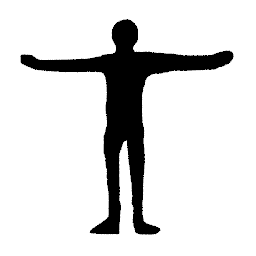
\includegraphics[width=0.92\linewidth]{img/person/target.png}
    \end{subfigure}
    \begin{subfigure}{0.23\textwidth}
        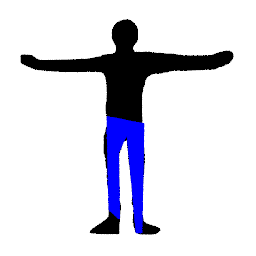
\includegraphics[width=0.92\linewidth]{img/person/iter_99.png}
    \end{subfigure}
    \caption{Placement of jeans on a human via the algorithm, matching conventional wisdom of where jeans belong on a human.}
    \label{fig:person}
\end{figure}

\begin{figure}
    \begin{subfigure}{0.23\textwidth}
        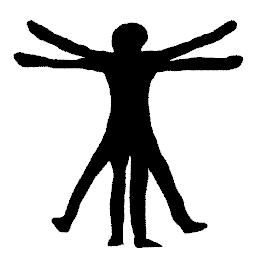
\includegraphics[width=0.92\linewidth]{img/vitruvian/target.png}
    \end{subfigure}
    \begin{subfigure}{0.23\textwidth}
        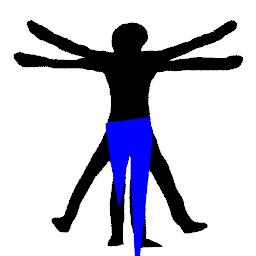
\includegraphics[width=0.92\linewidth]{img/vitruvian/iter_99.png}
    \end{subfigure}
    \caption{Placement of jeans on the Vitruvian Man, the body shape we all aspire to have.}
    \label{fig:vitruvian}
\end{figure}

\subsection{Novel Inputs}
We next tested the algorithm on a dog in an attempt to settle the original debate. The original image presented two hypotheses for dog jean placement: on the rear legs only, subdividing the dog into two horizontal sections, or on all legs, subdividing the dog into two vertical sections.~\cite{utopian_raspberry} Figure~\ref{fig:dog} shows that the algorithm places the jeans in a configuration much more like the latter than the former, but with a twist: rather than form-fitting the rear legs, the algorithm chose to collapse the rear pants leg so that it ends at the derri\`ere of the dog.

\begin{figure}
    \begin{subfigure}{0.23\textwidth}
        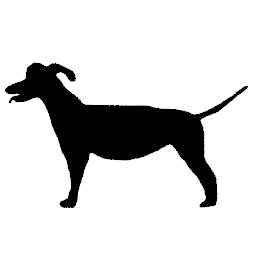
\includegraphics[width=0.92\linewidth]{img/dog/target.png}
    \end{subfigure}
    \begin{subfigure}{0.23\textwidth}
        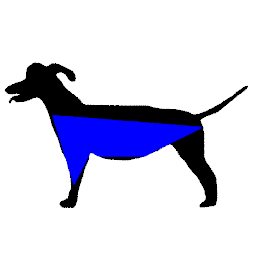
\includegraphics[width=0.92\linewidth]{img/dog/iter_99.png}
    \end{subfigure}
    \caption{Placement of jeans on a dog via the algorithm. The jeans are placed on all legs, but in an interesting deviation from the original hypothesis, the jeans leg for the rear legs has ridden up to align with the derri\`ere.}
    \label{fig:dog}
\end{figure}

In Figure~\ref{fig:others}, we present jeans applied to some more body shapes. First, one best described as horse-inspired (the literature shows that one likely cannot draw a good horse without reference material present~\cite{pagurek_2022}) dons a single pant leg. Here, the algorithm demonstrates that it would rather shrivel up a leg into nothing than stretch a waistband across any part of a horse. Next, a three-legged alien wears jeans on one and a half legs, with a small branch of jean reaching up to its shoulder for support. This demonstrates the algorithm's ability to balance its creative approach to jean design with functional concerns, like extra shoulder support. Finally, a spiky ball dragon wears jeans on only one of its ball legs, further demonstrating a preference for one-strapping.

\begin{figure}
    \begin{subfigure}{0.23\textwidth}
        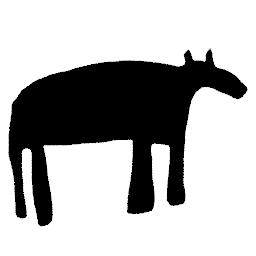
\includegraphics[width=0.92\linewidth]{img/horse/target.png}
    \end{subfigure}
    \begin{subfigure}{0.23\textwidth}
        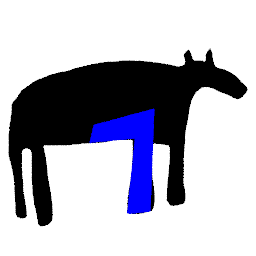
\includegraphics[width=0.92\linewidth]{img/horse/iter_99.png}
    \end{subfigure}

    \begin{subfigure}{0.23\textwidth}
        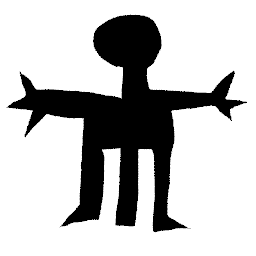
\includegraphics[width=0.92\linewidth]{img/tripod/target.png}
    \end{subfigure}
    \begin{subfigure}{0.23\textwidth}
        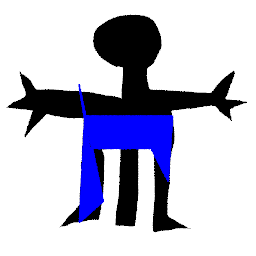
\includegraphics[width=0.92\linewidth]{img/tripod/iter_99.png}
    \end{subfigure}

    \begin{subfigure}{0.23\textwidth}
        
\includegraphics[width=0.92\linewidth]{img/balldragon/target.png}
    \end{subfigure}
    \begin{subfigure}{0.23\textwidth}
        
\includegraphics[width=0.92\linewidth]{img/balldragon/iter_99.png}
    \end{subfigure}
    
    \caption{Jean placements on alternative body shapes. Note the creative one-strap overall look of the tripod, and the bold asymmetric style of covering one ball of the ball dragon.}
    \label{fig:others}
\end{figure}

\section{Conclusion}
We have presented a mathematically sound optimization approach to determining the optimal configuration of pants on any object, should it choose to wear pants. Now that a definitive answer exists to this question, we expect no further arguments to be made on the subject on the internet. Since the algorithm's outputs are, by definition, optimal, one may choose to take lessons from its output, and begin casually rolling up just one pant leg in one's outfits.

\bibliographystyle{plainurl}
\bibliography{main}

\end{document}
